\documentclass[a4paper,12pt]{article}
\usepackage[utf8]{inputenc}
\usepackage[brazil]{babel}
\usepackage{amsmath}
\usepackage{amsfonts}
\usepackage{amssymb}
\usepackage{geometry}
\usepackage{graphicx}
\usepackage{xcolor}
\pagecolor[RGB]{5,40,97} % Define a cor de fundo da página
\color{white} % Define a cor do texto para branco

\geometry{
  a4paper,
  top=2cm,
  bottom=2cm,
  left=2cm,
  right=2cm,
}


\begin{document}

\title{Equações Fundamentais da Relatividade Geral h}
\author{}
\date{}

\begin{document}

\maketitle
\thispagestyle{empty}

\section*{Introdução}

A Relatividade Geral, formulada por Albert Einstein, é a teoria geométrica da gravitação e a descrição atual da gravidade na física moderna. Essencialmente, ela descreve a gravidade não como uma força, mas como uma curvatura do espaço-tempo causada pela massa e energia. As equações de campo de Einstein são o coração desta teoria, descrevendo como a matéria e a energia curvam o espaço-tempo.

\section{O Tensor de Einstein}

O tensor de Einstein ($G_{\mu\nu}$) descreve a curvatura do espaço-tempo. Ele é definido em termos do tensor de Ricci ($R_{\mu\nu}$) e do escalar de Ricci ($R$):

$$G_{\mu\nu} = R_{\mu\nu} - \frac{1}{2}g_{\mu\nu}R$$

onde $g_{\mu\nu}$ é o tensor métrico, que descreve a geometria do espaço-tempo.

\begin{figure}[h!] % [h!] tenta posicionar a imagem "aqui" (here)
    \centering % Centraliza o conteúdo dentro do ambiente figure
    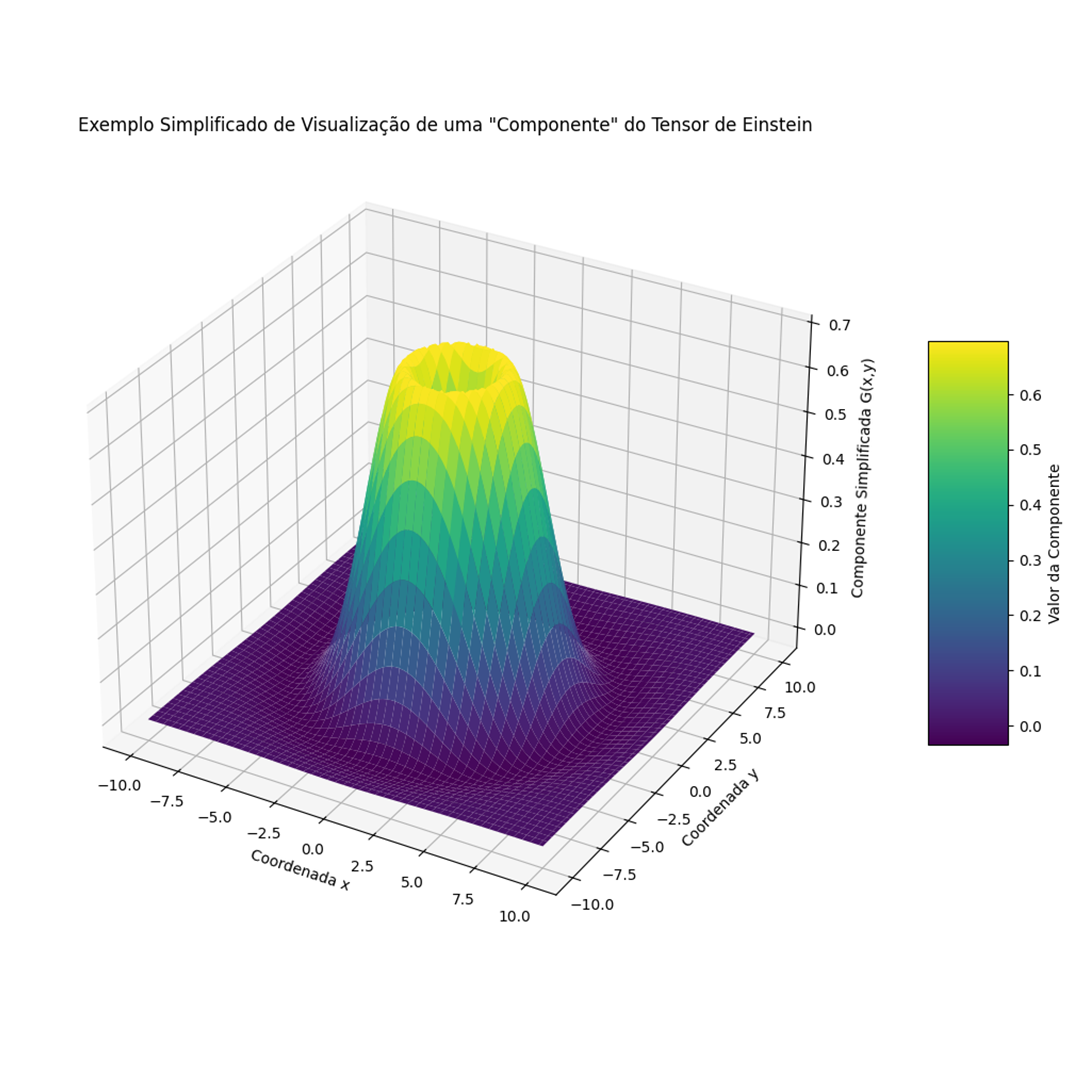
\includegraphics[width=0.5\textwidth]{Tensor_Einstein.png} % Ou .jpg, .pdf
    \caption{Versão Simplificada do Tensor.} % Legenda da imagem
    \label{fig:Tensor_Einstein} % Opcional: para referenciar a imagem no texto (e.g., Fig. \ref{fig:minha_imagem})
\end{figure}


\subsection{Tensor de Ricci}

O tensor de Ricci é obtido pela contração do tensor de Riemann ($R^\rho_{\mu\sigma\nu}$):

$$R_{\mu\nu} = R^\rho_{\mu\rho\nu}$$

O tensor de Riemann, por sua vez, é definido em termos das derivadas da conexão de Christoffel ($\Gamma^\lambda_{\mu\nu}$):

$$R^\rho_{\mu\sigma\nu} = \partial_\sigma \Gamma^\rho_{\mu\nu} - \partial_\nu \Gamma^\rho_{\mu\sigma} + \Gamma^\rho_{\kappa\sigma} \Gamma^\kappa_{\mu\nu} - \Gamma^\rho_{\kappa\nu} \Gamma^\kappa_{\mu\sigma}$$

\subsection{Escalar de Ricci}

O escalar de Ricci é obtido pela contração do tensor de Ricci com o tensor métrico:

$$R = g^{\mu\nu}R_{\mu\nu}$$

\subsection{Conexões de Christoffel}

As conexões de Christoffel, também conhecidas como símbolos de Christoffel do segundo tipo, são dadas por:

$$\Gamma^\lambda_{\mu\nu} = \frac{1}{2} g^{\lambda\sigma} \left( \partial_\mu g_{\nu\sigma} + \partial_\nu g_{\mu\sigma} - \partial_\sigma g_{\mu\nu} \right)$$

\section{As Equações de Campo de Einstein}

As equações de campo de Einstein relacionam a curvatura do espaço-tempo com a distribuição de massa e energia nele contida. Elas são escritas como:

$$G_{\mu\nu} = \frac{8\pi G}{c^4} T_{\mu\nu}$$

onde:
\begin{itemize}
	\item $G_{\mu\nu}$ é o tensor de Einstein.
	\item $G$ é a constante gravitacional de Newton.
	\item $c$ é a velocidade da luz no vácuo.
	\item $T_{\mu\nu}$ é o tensor de energia-momento, que descreve a densidade e o fluxo de energia e momento na matéria.
\end{itemize}

A constante $\frac{8\pi G}{c^4}$ é conhecida como a constante de acoplamento gravitacional.

\section{A Equação Geodésica}

As geodésicas representam o caminho de menor ação entre dois pontos no espaço-tempo curvo. Para partículas em queda livre sob a influência da gravidade, suas trajetórias seguem as geodésicas, descritas pela seguinte equação:

$$\frac{d^2x^\mu}{d\tau^2} + \Gamma^\mu_{\alpha\beta} \frac{dx^\alpha}{d\tau} \frac{dx^\beta}{d\tau} = 0$$

onde:
\begin{itemize}
	\item $x^\mu(\tau)$ são as coordenadas da partícula em função do tempo próprio $\tau$.
	\item $\Gamma^\mu_{\alpha\beta}$ são as conexões de Christoffel.
\end{itemize}

\section{O Tensor de Energia-Momento}

O tensor de energia-momento ($T_{\mu\nu}$) descreve o conteúdo de energia e momento do espaço-tempo. Sua forma específica depende do tipo de matéria ou campo presente. Por exemplo, para um fluido perfeito, o tensor de energia-momento é dado por:

$$T^{\mu\nu} = (\rho + \frac{p}{c^2}) u^\mu u^\nu - p g^{\mu\nu}$$

onde:
\begin{itemize}
	\item $\rho$ é a densidade de energia.
	\item $p$ é a pressão.
	\item $u^\mu$ é a quadrivelocidade do fluido.
\end{itemize}

\section{Conclusão}

As equações apresentadas aqui formam a base da Relatividade Geral, descrevendo a interação fundamental da gravidade como a curvatura do espaço-tempo causada pela presença de massa e energia. Estas equações têm implicações profundas para a nossa compreensão do universo, desde a dinâmica dos buracos negros e ondas gravitacionais até a evolução do próprio cosmos.

\end{document}